\section{Background}

\subsection{Explainable Artificial Intelligence}

Within XAI many methods have been developed to try to evaluate
ANN's, these methods are often referred as model interpretability methods.
In the field image recognition there has been a lot of work examining which
pixels of an image the model deems important. Arguably the most popular
method for this is Saliency Maps (CITE ME). There the pixel values the model
deems important are colored in s.t. a human can examine the image and get a
sense of what portions of the image are important to the model, an example of
a classification of a dog can be seen in Figure \ref{fig:dog_saliency}.

\begin{figure}[]
  \centering
  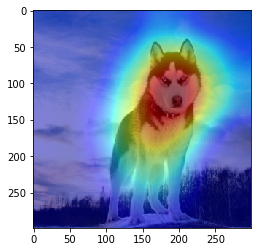
\includegraphics[width=.5\textwidth]{graphics/dog_saliency}
  \caption{Example of a models saliency map for an image of a dog}
  \label{fig:dog_saliency}
\end{figure}



\subsection{Reinforcement Learning}

In 2017 a Google based artificial intelligence research company published a paper called
`Mastering Chess and Shogi by Self-Play with a General Reinforcement Learning Algorithm`.
The paper described a Model based Reinforment learning agent and an accompanying Residual
Deep Neural Network architecture that was able to master the game of chess without being
given any idea of how to play the game of chess, and others. The architecture used in this
paper is heavily inspired by that architecture.

\subsection{Model Interpretability}

In 2018 the paper 'Interpretability Beyond Feature Attribution: Quantitative Testing with Concept Activation Vectors (TCAV)'
was published where an approach to model interpretability was introduced which is able to
distinguish

The deep neural network architecture that is used in this paper is based on the AlphaZero paper
published by DeepMind,
